\documentclass[a4paper, 11pt]{article}
\usepackage{doc}

\newcommand{\vfield}{\ensuremath{\bm{u}}}
\newcommand{\wfield}{\ensuremath{\bm{\omega}}}
\newcommand{\Fvfield}{\ensuremath{\hat{\bm{u}}}}
\newcommand{\position}{\ensuremath{\bm{x}}}
\newcommand{\nonlin}{\ensuremath{\bm{n}}}
\newcommand{\Fnonlin}{\ensuremath{\hat{\bm{n}}}}
\newcommand{\xhat}{\ensuremath{\hat{\bm{x}}}}
\newcommand{\yhat}{\ensuremath{\hat{\bm{y}}}}
\newcommand{\zhat}{\ensuremath{\hat{\bm{z}}}}
\newcommand{\wavenumber}{\ensuremath{\bm{k}}}
\newcommand{\posmeasure}{\ensuremath{\mathrm{d}\position}}
\newcommand{\pressure}{\ensuremath{p}}
\newcommand{\Fpressure}{\ensuremath{\hat{p}}}
\newcommand{\forcing}{\ensuremath{\bm{F}}}
\newcommand{\Fforcing}{\ensuremath{\hat{\bm{F}}}}
\newcommand{\production}{\ensuremath{\mathcal{P}}}
\newcommand{\dissipation}{\ensuremath{\varepsilon}}

\newcommand{\viscosity}{\ensuremath{\nu}}
\newcommand{\Reynolds}{\textit{Re}}

\newcommand{\Lx}{\ensuremath{L_x}}
\newcommand{\Ly}{\ensuremath{L_y}}
\newcommand{\Lz}{\ensuremath{L_z}}

\newcommand{\Nx}{\ensuremath{N_x}}
\newcommand{\Ny}{\ensuremath{N_y}}
\newcommand{\Nz}{\ensuremath{N_z}}

\newcommand{\dnsbox}{\texttt{dnsbox}}
\newcommand{\np}{\ensuremath{n_p}}
\newcommand{\kf}{\ensuremath{k_F}}
\newcommand{\nkf}{\ensuremath{n_F}}
\newcommand{\genf}{\ensuremath{f}}

% Some experimental macros
% convention:  \[type-of-the-variable][letter(s)][decorations]
% decorations: hat, bar, tilde, ... 

% scalars
\newcommand{\ubar}{\ensuremath{\overline{u}}}
\newcommand{\pbar}{\ensuremath{\overline{p}}}
\newcommand{\phibar}{\ensuremath{\overline{\phi}}}
\newcommand{\pRe}{\textit{Re}}
\newcommand{\dt}{\ensuremath{\Delta t}}

% vectors
\newcommand{\vu}{\ensuremath{\bm{u}}}
\newcommand{\vuhat}{\ensuremath{\hat{\vu}}}
\newcommand{\vuhatbar}{\ensuremath{\bar{\vuhat}}}
\newcommand{\vubar}{\ensuremath{\overline{\vu}}}
\newcommand{\vubarhat}{\ensuremath{\hat{\vubar}}}
\newcommand{\vf}{\ensuremath{\bm{f}}}
\newcommand{\vfbar}{\ensuremath{\overline{\bm{f}}}}
\newcommand{\vk}{\ensuremath{\bm{k}}}
\newcommand{\vx}{\ensuremath{\bm{x}}}
\newcommand{\vz}{\ensuremath{\bm{z}}}
\newcommand{\vy}{\ensuremath{\bm{y}}}
\newcommand{\vxhat}{\ensuremath{\hat{\vx}}}
\newcommand{\vzhat}{\ensuremath{\hat{\vz}}}
\newcommand{\vyhat}{\ensuremath{\hat{\vy}}}


% Matrices/Tensors
\newcommand{\Sbar}{\ensuremath{\overline{S}}}
\newcommand{\tSbar}{\ensuremath{\overline{\bm{S}}}}

% Operators
\renewcommand{\d}{\partial}
\newcommand{\oF}{\ensuremath{\mathcal{F}}}
\newcommand{\oL}{\ensuremath{\mathcal{L}}}
\newcommand{\oN}{\ensuremath{\mathcal{N}}}
\newcommand{\con}{\ensuremath{\ast}}

% Symbols
\newcommand{\oo}{\ensuremath{\infty}}
\newcommand{\<}{\ensuremath{\leftarrow}}
\renewcommand{\>}{\ensuremath{\rightarrow}}

% Greek letters
\newcommand{\al}{\alpha}
\newcommand{\AL}{\Alpha}
\newcommand{\be}{\beta}
\newcommand{\BE}{\Beta}
\newcommand{\ga}{\gamma}
\newcommand{\GA}{\Gamma}
\newcommand{\de}{\delta}
\newcommand{\DE}{\Delta}
\newcommand{\ep}{\epsilon}
\newcommand{\EP}{\Epsilon}
\newcommand{\ze}{\zeta}
\newcommand{\ZE}{\Zeta}
\newcommand{\et}{\eta}
\newcommand{\ET}{\Eta}
\renewcommand{\th}{\theta}
\renewcommand{\TH}{\Theta}
\newcommand{\ka}{\kappa}
\newcommand{\KA}{\Kappa}
\newcommand{\la}{\lambda}
\newcommand{\LA}{\Lambda}
\newcommand{\rh}{\rho}
\newcommand{\RH}{\Rho}
\renewcommand{\si}{\sigma}
\renewcommand{\SI}{\Sigma}
\newcommand{\ta}{\tau}
\newcommand{\TA}{\Tau}
\newcommand{\ph}{\phi}
\newcommand{\PH}{\Phi}
\newcommand{\om}{\omega}
\newcommand{\OM}{\Omega}
\newcommand{\ch}{\chi}
\newcommand{\CH}{\Chi}
\newcommand{\ps}{\psi}
\newcommand{\PS}{\Psi}

\bibliography{doc}

\title{dnsbox}
\date{13 July 2021}
\author{Gökhan Yalnız\\\href{mailto:gokhan.yalniz@ist.ac.at}{
                             gokhan.yalniz@ist.ac.at}
        \and
        Nazmi Burak Budanur\\\href{mailto:nbudanur@pks.mpg.de}{
                                   nbudanur@pks.mpg.de}}

\hypersetup{
    pdftitle={dnsbox},
    pdfauthor={Gökhan Yalnız, Nazmi Burak Budanur}
}


\begin{document}
\maketitle

\section{Equations and geometry} 

\dnsbox\ simulates the nondimensionalized Navier--Stokes equation 
\begin{equation}
    \vu_t = -(\vu \cdot \nabla) \vu - \nabla p
    + \pRe^{-1} \nabla^2 \vu + \vf \,, \label{NSe}
\end{equation}
where the velocity field \vu\ is subject to the incompressibility condition 
\begin{equation}
    \nabla \cdot \vu = 0\,, \label{incompressibility}
\end{equation}
and the periodic boundary conditions 
\begin{equation}
    \vu(x,y,z) = 
    \vu(x + \Lx, y, z) = \vu(x, y + 4, z) = \vu(x, y, z + \Lz) \,. \label{boundary_conditions}
\end{equation}
Currently, three body force terms 
\begin{equation}
    \vf_0 = 0 \,,\quad
    \vf_1 = (4 \pRe)^{-1} \pi^{2} \sin(\pi y / 2) \xhat \,,\quad
    \vf_2 = (4 \pRe)^{-1} \pi^{2} \cos(\pi y / 2) \xhat 
\end{equation}
are supported through the \texttt{forcing} parameter. The option to 
choose between \(\vf_1\) and \(\vf_2\) is a convenience: while switching 
between the two is physically equivalent to a quarter-domain translation in \(y\),
the code implements reflection in \(y\) (among many other symmetry operations),
which picks an origin for \(y\).

For \(\vf_1\) we find the laminar solution
\begin{equation} 
    \vu_l = \sin(\pi y / 2) \xhat \label{laminar}
\end{equation}
with unit amplitude. As seen, the amplitude of this solution is used
as the velocity scale and its peak location $y_p=1$ as the length scale, yielding 
the Navier--Stokes equation \cref{NSe} with the single control parameter $\pRe$. 

\section{Spatial discretization}
The spatial discretization is performed by truncating the Fourier series
\begin{equation}
    \vu(x, y, z) = 
        \sum_{q_x = -\infty}^{\infty}
        \sum_{q_y = -\infty}^{\infty}
        \sum_{q_z = -\infty}^{\infty}
        \vuhat (q_x, q_y, q_z)
        e^{i 2\pi (q_x x / L_x + q_y y / L_y + q_z z / L_z)} 
        \label{fourier_series}
\end{equation}
to retain 
\begin{align}
    q_x &= -n_x / 2 + 1, \ldots n_x / 2 - 1 \,, \\
    q_y &= -n_y / 2 + 1, \ldots n_y / 2 - 1 \,, \\
    q_z &= -n_z / 2 + 1, \ldots n_z / 2 - 1 \,,
\end{align}
resulting in an equivalent $n_x \times n_y \times n_z$-dimensional
\footnote{Nyquist modes \(q_x=n_x /2\), \(q_y=n_y/2\) and \(q_z=n_z/2\) are zeroed.}
 spatial
grid.
Since $\vu (x,y,z)$ is real valued, we exploit 
$\vuhat (q_x, q_y, q_z) = \vuhat^* (- q_x, - q_y, - q_z) $ and hold only 
\begin{align}
    q_x &= -n_x / 2 + 1, \ldots n_x / 2 - 1 \,, \\
    q_y &= 0, \ldots n_y / 2 - 1 \,, \\
    q_z &= -n_z / 2 + 1, \ldots n_z / 2 - 1 \,.
\end{align}
in memory. 

We define the wave vectors
\begin{equation}
    \vk[q_x, q_y, q_z] = \alpha q_x \xhat + \beta q_y \yhat + \gamma q_z \zhat \,, 
\end{equation}
where $\alpha = 2 \pi / L_x \,, \beta = \pi / 2 \,, \gamma = 2 \pi / L_z$, which allows 
us to rewrite \cref{fourier_series} compactly as 
\begin{equation}
    \vu (\vx) = \sum_{\vk} \vuhat (\vk) e^{i \vk \cdot \vx} \, .
\end{equation}

\section{Evaluation of the nonlinear term}

We evaluate the nonlinear term of \cref{NSe} pseudospectrally in
its divergence form $\nabla \cdot (\vu \vu^T)$ on a grid that is $3/2$ denser than 
our original grid in order to avoid aliasing errors. The supersampled grid dimension 
is therefore $3n_x/2 \times 3n_y/2 \times 3n_z/2$. 

\section{Temporal discretization}

Time stepping is performed by a semi-implicit predictor-corrector method which we
adapted from \href{openpipeflow.org}{\texttt{openpipeflow}} \cite{willis2017openpipeflow} 
and describe here. In the Fourier space, the Navier--Stokes equations 
\cref{NSe} can be brought to the form 
\begin{equation}
    \d_t \vuhat = \oL \vuhat + \oN (\vuhat) \label{eq_time_step}
\end{equation}
where $\oL = - \pRe^{-1} \|\vk\|^2 $, 
$\oN (\vuhat) = \oF\{ -(\vu \cdot \nabla) \vu - \nabla p + \vf \}$, 
and $\nabla^2 p = -\nabla \cdot (\vu \cdot \nabla) \vu$. 
Denoting the time step by $\DE t$ and 
the present and next fluid states 
by $\vuhat_i$ and $\vuhat_{i + 1}$, respectively, 
we approximate \cref{eq_time_step} as 
\begin{equation}
    \frac{\vuhat_{i+1} - \vuhat_i}{\Delta t} 
    = \theta \oL  \vuhat_{i+1}  + (1 - \theta) \oL  \vuhat_i
    + \theta \oN (\vuhat_{i+1}) + (1 - \theta) \oN (\vuhat_i) ,
    \label{semi_implicit_time_step}
\end{equation}
where the parameter $\theta$ is called ``implicitness''. 
Reorganizing the terms in \cref{semi_implicit_time_step}, we get an 
expression for the next time step as 
\begin{equation}
   (\DE t^{-1} - \theta \oL ) \vuhat_{i+1} = 
    \DE t^{-1} \vuhat_i +  (1 - \theta) (\oL  \vuhat_i + \oN (\vuhat_i)) + \theta \oN (\vuhat_{i+1})
    \label{state_next}
\end{equation}
In order to get to the next time step, we solve the equation above by a fixed-point iteration
\begin{equation}
    (\DE t^{-1} - \theta \oL ) \vuhat_{i+1}^{c+1} = 
    \DE t^{-1} \vuhat_i 
    +  (1 - \theta) (\oL  \vuhat_i 
    + \oN (\vuhat_i)) + \theta \oN (\vuhat_{i+1}^{c}) \,, \label{corrector}
\end{equation}
which are also known as the ``corrector iterations''. To be able to initiate this, we need 
a prediction, which we obtain by treating the nonlinear term explicitly as
\begin{equation}
    (\DE t^{-1} - \theta \oL ) \vuhat_{i+1}^0 = 
    \DE t^{-1} \vuhat_i +  (1 - \theta) \oL  \vuhat_i + \oN (\vuhat_i) \,. \label{predictor}
\end{equation}
The corrector iterations \cref{corrector} somewhat simplify when written for the 
corrections $\Delta \vuhat^{c + 1} = \vuhat_{i+1}^{c+1} - \vuhat_{i+1}^{c}$
\begin{equation}
    (\DE t^{-1} - \theta \oL )\, \Delta \vuhat^{c + 1} =  
    \theta ( \oN (\vuhat_{i + 1}^{c}) - \oN (\vuhat_{i + 1}^{c - 1}) ) \label{correction}
\end{equation}
with $\oN (\vuhat_{i + 1}^{- 1}) \equiv  \oN (\vuhat_{i})$. Our time stepping code begins 
with \cref{predictor} then iterates \cref{correction} along with 
$\vuhat_{i+1}^{c+1} = \vuhat_{i+1}^{c} + \Delta \vuhat^{c + 1}$ until
$\| \Delta \vuhat^{c + 1} \| / \| \vuhat_{i + 1}^{0} \| < \mbox{\texttt{steptol}}$  

\section{Parallelization}

When run in parallel, \dnsbox\ distributes $\vuhat [q_x, q_y, q_z]$ in the $q_x$ direction 
and $\vu (x, y, z)$ in the $z$-direction to $n_p$ processors. It is necessary to have 
$n_x / n_p$ an integer greater than $1$ and $n_x$ divisible by $n_p$. Although the same 
condition is not required for 
$n_z / n_p$, optimal performance is achieved when it is the case.

\section{Symmetries}

Several symmetry operations are implemented in the \texttt{symmops} module of 
\dnsbox . These are the shifts
\begin{align}
   T_x (s_x) \vu (x, y, z) &= \vu (x - s_x, y, z) \,, \\
   T_y (s_y) \vu (x, y, z) &= \vu (x, y - s_y, z) \,, \\
   T_z (s_z) \vu (x, y, z) &= \vu (x, y, z - s_z) \,,
\end{align}
reflections 
\begin{align}
    \sigma_x [u, v, w](x, y, z) &= [-u, v, w](-x, y, z) \,, \\
    \sigma_y [u, v, w](x, y, z) &= [u, -v, w](x, -y, z) \,, \\
    \sigma_z [u, v, w](x, y, z) &= [u, v, -w](x, y, -z) \,,
\end{align}
half-domain shifts 
\begin{align}
    T_{x/2} = T_x (L_x / 2)\,, T_{y/2} = T_y (L_y / 2)\,, T_{z/2} = T_z (L_z / 2)\,, 
\end{align}
and composite transformations
\begin{align}
    S_x = \sigma_x T_{y/2}\,,\quad
    S_y = \sigma_y T_{y/2} \quad\mbox{and}\quad 
    R_{xy} = \sigma_x \sigma_y \, .
\end{align}
Note that the specific form of $\vf$ might not be compatible with some of these symmetries. In other words,
it is not guaranteed that if $\vu$ is a solution, then its transformed version $g \vu$ is also one, 
where $g$ is one of the operators above. Invariance under a subset of the discrete symmetries 
can be enforced throughout the simulation by specifying it in the \texttt{parameters.in} file. 

\section{Code validation}

\texttt{make test} runs module tests of \dnsbox\ and validates the time stepper
against the ``Shapiro solution'' \cite{shapiro1993use}
\begin{align}
    u &= -  \exp (- \lambda^2 t / Re) (\alpha^2 + \beta^2)^{-1} \nonumber \\
      & \times [\lambda \beta \cos(\alpha x) \sin (\beta y) \sin (\gamma z) 
             + \gamma \alpha \sin(\alpha x) \cos (\beta y) \cos (\gamma z)] \,, \nonumber \\
    v &= \exp (- \lambda^2 t / Re) (\alpha^2 + \beta^2)^{-1} \nonumber \\
    & \times [\lambda \alpha \sin(\alpha x) \cos (\beta y) \sin (\gamma z) 
        - \gamma \beta \cos(\alpha x) \sin (\beta y) \cos (\gamma z)] \,, \label{shapiro_solution}\\
    w &= \exp (- \lambda^2 t / Re) \cos(\alpha x) \cos (\beta y) \sin (\gamma z) \,, \nonumber
\end{align}
where $\lambda = \sqrt{\alpha^2 + \beta^2 + \gamma^2}$.  \cref{shapiro_solution} is an 
analytical solution of \cref{NSe} for $\vf = 0$.

\section{Large eddy simulation}

In our implementation of large eddy simulation (LES), we closely follow
\cite{pope2000turbulent} and \cite{vanVeen2018transitions} 
and essentially adapt the latter's formulation to \dnsbox\ conventions.
Let $G$ be the kernel of an LES filter action of which is given by the 
convolution
\begin{equation}
    \phibar = G \con \vu = 
    \int_{-\oo}^{\oo} \int_{V} \phi (\vx', t') 
                                G(\vx - \vx', t - t') dt' d\vx' 
    \,. \label{les_filter}
\end{equation} 
Applying this filter on the Navier--Stokes equations \cref{NSe} results 
in the linear terms of the same form. Using the index notation where repeated 
indices imply summation, we can write the filtered advection term as 
\begin{equation}
    \overline{u_i \d_i u_j} 
      = \d_i \overline{u_i u_j}
      = \d_i (\ubar_i \ubar_j) + \d_i (\overline{u_i u_j} - \ubar_i \ubar_j)
      = \ubar_i \d_i \ubar_j + \d_i \tau_{ij}^{R} \,,
\end{equation}
where $\tau_{ij}^{R}$ is the \emph{residual stress tensor}. Noting that this 
tensor can be decomposed as
\begin{equation}
    \tau_{ij}^{R} = \frac{1}{3} \tau_{kk} \delta_{ij} + \tau_{ij}^{r}
    \label{residual_stress_tensor}
\end{equation}
we write the filtered Navier--Stokes equations as 
\begin{equation}
	\d_t \ubar_j = 
        -\ubar_i  \d_i \ubar_j - \d_i \tau_{ij}^r - \d_j \pbar 
        + \pRe^{-1} \d_i \d_i \ubar_j + \vfbar \, . 
        \label{filtered_NSe}
\end{equation}
We absorbed the isotropic part of the
residual stress tensor \cref{residual_stress_tensor} into the filtered
pressure, i.e. $\pbar \< \pbar + \tau_{kk} / 3 $. 

All terms in the filtered
Navier--Stokes equations \cref{filtered_NSe}, except the anisotropic residual
stress tensor $\tau_{ij}^r$ are in terms of filtered fields $\vubar$ and
$\pbar$. Thus, in order to close \cref{filtered_NSe}, we need a model of
$\tau_{ij}^r$ in terms of the filtered fields, i.e. a closure. Here, we
implement the Smagorinsky model 
\begin{equation}
    \tau_{ij}^r = - 2 \nu_t \Sbar_{ij} 
\end{equation}
where  
\begin{equation}
    \Sbar_{ij} = (\d_i \ubar_j + \d_j \ubar_i) / 2
\end{equation}
is \emph{the filtered rate-of-strain tensor}, 
\begin{equation}
    \nu_T = (C_S \Delta)^2 \sqrt{2 \Sbar_{ij} \Sbar_{ij}}
    \label{eddy_viscosity}
\end{equation}
is \emph{the eddy viscosity}, $C_S$ is called the Smagorinsky constant  and
$\Delta = \Lx / n_x$ is the shortest resolved length scale. With this closure, 
we write the final LES equations
\begin{equation}
	\d_t \ubar_j = 
        -\ubar_i  \d_i \ubar_j - \d_j \pbar 
        + 2 \d_i (\pRe^{-1} + \nu_T) \Sbar_{ij} + \vfbar \, , 
        \label{LES}
\end{equation}
which we simulate under the incompressibility condition $\d_i \ubar_i = 0$ 
and periodic boundaries $\ubar|_{x_i} = \ubar|_{x_i + L_i}$.

In order to time step LES equations \cref{LES}, we write them in the form
\begin{equation}
    \d_t \vubarhat = \oL \vubarhat + \oN (\vubarhat) \label{eq_time_step_LES}
\end{equation}
where
\begin{eqnarray}
    \vubarhat &=& \oF \{ \vubar \}   \,, \label{Fourier} \\
    \oL &=& - \pRe^{-1} \| \vk \|^2  \,, \label{oL} \\ 
    \oN (\vubarhat) &=& \oF \{- (\vubar \cdot \nabla) \vubar 
                              - \nabla \pbar 
                              + \vfbar
                              + 2 \nabla \nu_T \tSbar \} \, . \label{oN}
\end{eqnarray}
Since the linear term \cref{oL} is identical in the DNS, at the code level, 
LES is implemented by varying the nonlinear term according to \cref{oN}
and \cref{eddy_viscosity}.

We tested the LES implementation by comparing the resulting states against those 
from DNS. Fig. \ref{les_dns} shows the energy spectra and velocity profiles of 
states obtained from DNS with $n_{x,y,z} = 256$ and LES with $n_{x,y,z} = 64$
and $n_{x,y,z} = 32$ at $\pRe = 20,000$. The test shows reasonable agreement, 
which could probably be improved by collecting statistics. As of this writing, 
we have not yet attempted this. 

\begin{figure}
    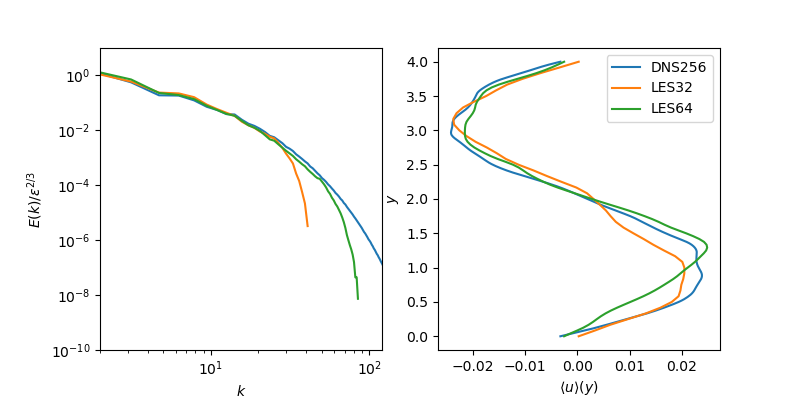
\includegraphics[width=\textwidth]{dns_les.png}
    \caption{Energy spectrum (left) and velocity profiles (right) obtained from 
    DNS and LES at $\pRe = 20,000$. \label{les_dns}}
\end{figure}

\printbibliography
\end{document}
